\part{Physical Prototyping}
\frame{\partpage}

\begin{frame}{Intro}
	\begin{itemize}
		\item Are the easiest for designers to construct
		\item Usually created from 
		\begin{itemize}
			\item hand-drawn items
			\item found objects
			\item boardgame pieces
		\end{itemize}
	\end{itemize}
\end{frame}

\begin{frame}
	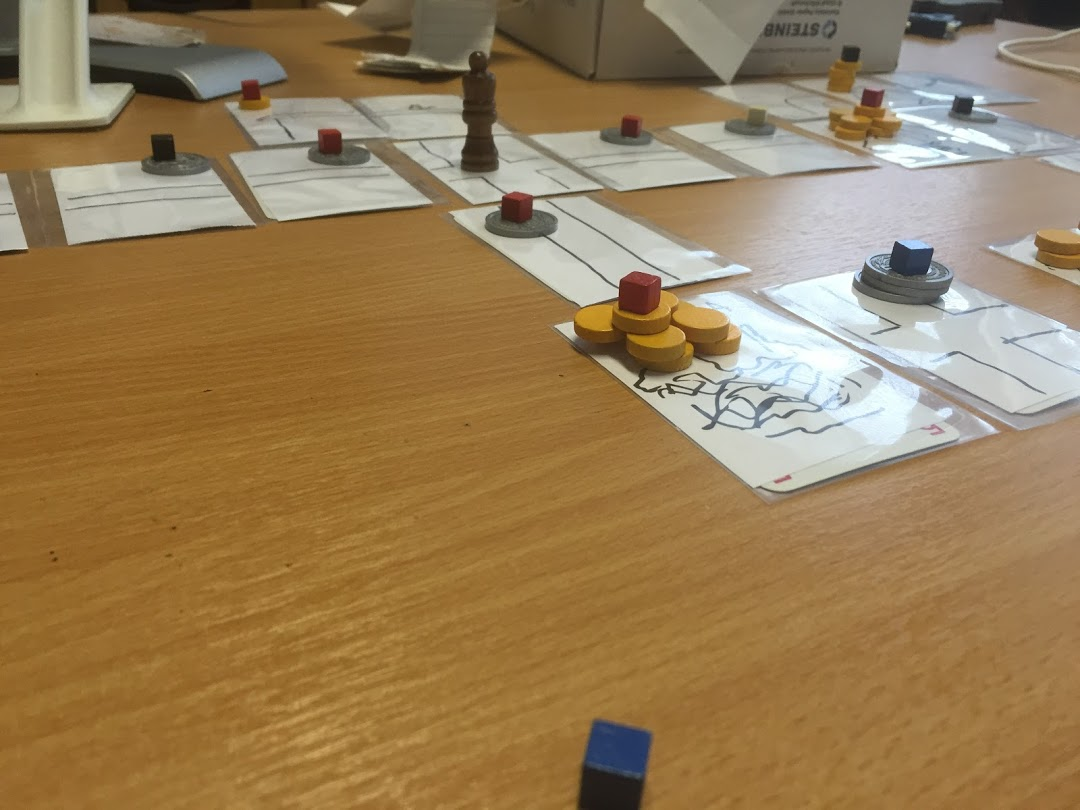
\includegraphics[width=1.0\textwidth]{board_game_prototype}
\end{frame}

\begin{frame}
	\begin{itemize}
		\item Two approaches
		\begin{itemize}
			\item Focus on gameplay (see below)
			\item Mock up what the game would play like
		\end{itemize}
	\end{itemize}
\end{frame}

\begin{frame}{Benefits of Paper}
	\begin{itemize}
		\item Allows you to focus on gameplay rather than technology
		\item Easier to iterate
		\item Easier to amend, can respond in real time to player feedback
	\end{itemize}
\end{frame}

\begin{frame}{Physical Prototyping Hints}
	\begin{itemize}
		\item In early iterations pay no attention to art work
		\item Build a representation of your core gameplay
		\item Designing the space (board) will give you an idea how your units will move
		\item Designing basic objects will help you build relationships in your game
		\item Try to keep the ruleset simple, only add a rule to make the gameplay playable
	\end{itemize}
\end{frame}

\begin{frame}{Physical Prototyping Issues}
	\begin{itemize}
		\item Not great for tracking lots of information
		\item Game rhythm issues, physical prototypes tend to have a rigid turn structure
		\item Difficult to prototype Kinesthetics
	\end{itemize}
\end{frame}
